%-*-coding: utf-8;-*-
\documentclass[italian,a4paper,hidelinks,headinclude]{scrartcl}
\usepackage{amsmath,amssymb,amsthm,thmtools}
\usepackage{eucal,babel,a4}
\usepackage[nochapters,pdfspacing]{classicthesis}
\usepackage[utf8]{inputenc}
\usepackage{graphicx,caption,subcaption}
\usepackage{bussproofs}
\usepackage{comment}
\usepackage{xcolor}
\usepackage{tikz,fancybox}

\newcommand{\NN}{{\mathbb N}}
\newcommand{\ZZ}{{\mathbb Z}}
\newcommand{\QQ}{{\mathbb Q}}
\newcommand{\RR}{{\mathbb R}}
\newcommand{\CC}{{\mathbb CC}}
\newcommand{\C}{{\mathcal C}}
\newcommand{\F}{{\mathcal F}}
\renewcommand{\P}{{\mathcal P}}
\newcommand{\defeq}{=}
\DeclareMathOperator{\diag}{diag}
\newcommand{\myemph}[1]{\emph{#1}\marginpar{#1}}

\def\Xint#1{\mathchoice
{\XXint\displaystyle\textstyle{#1}}%
{\XXint\textstyle\scriptstyle{#1}}%
{\XXint\scriptstyle\scriptscriptstyle{#1}}%
{\XXint\scriptscriptstyle\scriptscriptstyle{#1}}%
\!\int}
\def\XXint#1#2#3{{\setbox0=\hbox{$#1{#2#3}{\int}$ }
\vcenter{\hbox{$#2#3$ }}\kern-.6\wd0}}
\def\dashint{\Xint-}

\declaretheoremstyle[
spaceabove=6pt, spacebelow=6pt,
headfont=\normalfont\itshape,
notefont=\mdseries, notebraces={(}{)},
bodyfont=\normalfont,
postheadspace=1em,
qed=,
shaded={rulecolor=pink!30,rulewidth=1pt,bgcolor=pink!10}
]{mystyle}

\declaretheorem[numberwithin=section,name=Teorema]{theorem}
\declaretheorem[sibling=theorem,name=Definizione]{definition}
\declaretheorem[sibling=theorem,name=Lemma]{lemma}
\declaretheorem[style=mystyle,sibling=theorem,name=Esercizio]{exercise}
\declaretheorem[style=mystyle,sibling=theorem,name=Esempio]{example}
\declaretheorem[sibling=theorem,name=Paradosso]{paradox}

\begin{document}
\title{Cenni di logica e teoria degli insiemi
\thanks{%
Puoi scaricare o contribuire a questi appunti su
\url{https://github.com/paolini/appunti/}}}
\author{E. Paolini}

\maketitle

\section{Sistemi formali}
Fin dai tempi di Aristotele si è cercato di individuare e descrivere
le leggi che governano la \emph{deduzione}. Si è osservato che
combinando tra loro singole informazioni è possibile estrarre da esse
nuove informazioni che in origine non erano disponibili. Ad esempio
dalle due informazioni
\begin{align*}
  (P) & \qquad \textit{in ogni triangolo isoscele gli angoli alla base
    sono uguali}\\
  (Q) & \qquad \textit{questo triangolo è
    isoscele}
\end{align*}
si può dedurre
\begin{align*}
  (R) \qquad \textit{gli angoli alla base di
    questo triangolo sono uguali.}
\end{align*}
Quello che abbiamo fatto è una
\emph{deduzione} (anche detta \emph{derivazione}).
Nelle notazioni dei \myemph{sistemi formali}
$P,Q,R$ si chiamano \myemph{formule}.
Una volta aggiunta $R$ alle informazioni note, si potranno fare
ulteriori derivazioni in cui oltre a $P$ e $Q$ si potrà usare anche
$R$. Questo permette di estendere l'insieme delle conoscenze, a
partire da un nucleo iniziale di conoscenze primitive che chiameremo
\myemph{assiomi}.

Le regole che ci permettono di passare da una o più formule ad una
nuova formula, si chiamano \myemph{regole di inferenza}. Normalmente le
formule sono composte da una sequenza di \myemph{simboli} che possono
essere scelti tra lettere, cifre o altro. Eventualmente una
\myemph{grammatica} determinerà come i simboli possono essere utilizzati
per comporre le formule (in tal caso le sequenze ammissibili vengono
chiamate \myemph{formule ben formate}). Le regole di inferenza
devono essere le più semplici possibile, di preferenza dovrebbero
essere delle regole \emph{meccaniche} in modo che non ci possano
essere dubbi su come vadano applicate.

Nell'esempio che abbiamo fatto all'inizio del paragrafo le formule (P), (Q) e (R)
sono espresse nel \myemph{linguaggio naturale} ovvero nella lingua che
siamo abituati ad utilizzare ogni giorno. Formalizzare il linguaggio
naturale risulta un compito improbo: sono troppe le ambiguità, i
sottointesi, le interpretazioni soggettive, perché si possa pensare di
trovare le regole di inferenza di tale linguaggio. Quello che si può fare è
costruire un \myemph{linguaggio artificiale} che sia  sufficientemente
semplice da poter essere formalizzato in modo non ambiguo. Normalmente
il linguaggio artificiale sarà comunque ispirato al linguaggio
naturale. E' però possibile costruire dei linguaggi che non abbiano
niente a che fare con la lingua naturale, e questo può essere un utile
esercizio perché ci mette nella situazione di non poter dare un significato
alle formule e di doversi quindi ciecamente e meccanicamente affidare
alle regole formali di inferenza. Lo facciamo nel seguente
esempio\footnote{%
  Esempio tratto dal libro
    \emph{G\"odel, Escher, Bach: un'eterna ghirlanda brillante} di
    Douglas Hofstadter}.

\begin{example}[sistema \texttt{MIU}]
Prendiamo come simboli le lettere: \texttt{MIU}.
Consideriamo ben formate tutte
le formule composte da una sequenza di queste lettere. Ad esempio
saranno formule ben formate: \texttt{UMI, MIMMI, IMMUMMMIIUMI}. Come
regole di inferenza consideriamo le seguenti:
\begin{enumerate}
\item  $x$\texttt{I} $\to$ $x$\texttt{IU} (cioé: si può aggiungere una
  \texttt{U} alla fine delle formule che terminano con \texttt{I})
\item \texttt{M}$x$ $\to$ \texttt{M}$xx$ (cioé: si può raddoppiare la
  sequenza di simboli dopo una \texttt{M} iniziale)
\item $x$\texttt{III}$y$ $\to$ $x$\texttt{U}$y$ (cioé: si può
  rimpiazzare ogni sequenza \texttt{III} con \texttt{U})
\item $x$\texttt{UU}$y$ $\to$ $xy$ (cioé: si può rimuovere la sequenza \texttt{UU}).
\end{enumerate}
Ecco un esempio di derivazione a partire dalla formula \texttt{MIIMI}:
\begin{center}
  \begin{tabular}{l}
    \texttt{MIIMI} (ipotesi)\\\hline
    \texttt{MIIMIIIMI} (regola 2.)\\
    \texttt{MIIMUMI} (regola 3.)\\
    \texttt{MIIMUMIU} (regola 1.)\\
  \end{tabular}
\end{center}

A partire dalla formula \texttt{MI} è possibile derivare la formula \texttt{MU}?
\end{example}

\marginpar{sistema \texttt{IVXPU}}
\begin{example}
Si  considerino le formule formate dai simboli
\texttt{IVXPU}.
Si prendano le seguenti regole di inferenza:
  \begin{enumerate}
  \item $x$\texttt{P}$y$\texttt{U}$z$ $\to$ $x$\texttt{IP}$y$\texttt{U}$zy$,
  \item $x$\texttt{P}$y$\texttt{U}$z$ $\to$ $x$\texttt{P}$y$\texttt{IU}$zx$,
  \item $x$\texttt{IIIII}$y$ $\to$ $x$\texttt{V}$y$,
  \item $x$\texttt{VV}$y$ $\to$ $x$\texttt{X}$y$.
  \end{enumerate}
  Si prenda come assioma: \texttt{IPIUI}. Si riesce ad ottenere la formula \texttt{VPVUXXV}?
\end{example}

Per risolvere la richiesta precedente probabilmente è
necessario trovare una \emph{interpretazione} dei simboli
utilizzati. Si provi a immaginare che i simboli \texttt{IVX}
rappresentino numeri romani... come vanno interpretati i simboli
\texttt{PU} per dare un senso comune alle formule del sistema
\texttt{IVXPU}?

\section{Modello, verità, completezza}

Nel sistema formale \texttt{IVXPU}
che abbiamo considerato nel paragrafo precedente i simboli possono essere interpretati
come operazioni su numeri naturali. Si dice allora che l'insieme dei
numeri naturali fornisce un \myemph{modello} per questo sistema
formale. Il modello associa un valore di \myemph{verità} ad ogni formula.
Se ogni assioma viene interpretato come un fatto vero, e ogni regola
formale mantiene il valore di \emph{verità} delle formule (cioè
partendo da una formula vera e applicando una qualunque regola formale
si ottiene un'altra formula vera) allora ogni derivazione del sistema
formale produce sicuramente formule vere.

Nel nostro caso l'assioma \texttt{IPIUI} corrisponde alla verità:
$1\cdot 1 = 1$ e
la prima regola di inferenza corrisponde alla seguente verità:
\[
\text{se $x\cdot y = z$ allora $(x+1)\cdot y = z + y$.}
\]
E' dunque chiaro che ogni formula ottenuta con questo sistema formale
sarà interpretata come vera. Ci chiediamo: è possibile, in questo
sistema, derivare qualunque formula vera? La risposta è negativa
in quanto si può osservare che la formula: \texttt{VIUIIIPII} potrebbe
essere interpretata come $6 = 3\cdot 2$ che è vera, ma non può essere
dimostrata mediante le regole formali che abbiamo scelto.
In questo caso si dice che il sistema è \myemph{incompleto} in quanto ci sono
formule vere che non possono essere dimostrate.

Si potrebbero aggiungere delle regole \emph{grammaticali}
per mettere dei vincoli su quali siano le formule ben formate. Si
potrebbe ad esempio richiedere che la formula contenga una sola
\texttt{P} e una sola \texttt{U} e che la \texttt{P} si trovi sempre
prima della \texttt{U}. In questo modo si escludono tutte le formule
vere che non posso essere derivate e il sistema si dice \emph{completo}.
Il concetto di \myemph{completezza} è fondamentale per capire il significato
del teorema di G\"odel, di cui parleremo brevemente più avanti.





\section{Logica delle proposizioni}

Nella \emph{logica delle proposizioni} si aggiunge il concetto di
\emph{verità} all'interno del sistema formale.
Le formule prendono il nome di \myemph{proposizioni} e possono assumere un valore
di verità:
\texttt{V}=\myemph{vero} o \texttt{F}=\myemph{falso}.
Si introducono quindi i \myemph{connettivi logici} ovvero gli operatori
$\neg$ (negazione: non), $\land$ (congiunzione: e), $\lor$ (disgiunzione:
o), $\Rightarrow$ (implicazione: solo se), $\Leftarrow$ (implicazione
inversa: se), $\Leftrightarrow$ (doppia implicazione: se e solo se) che
applicati ad una (per la negazione) o due proposizioni (per tutti gli altri
connettivi) producono una nuova proposizione il cui valore di verità
può essere meccanicamente dedotto dal valore di verità delle
proposizioni a cui è stato applicato. Essendoci solo un numero finito di
combinazioni, possiamo definire le operazioni logiche elencando, in
forma di tabella, tutti i valori possibili che possono assumere una
coppia di proposizioni $P$ e $Q$ e i corrispondenti valori per le
varie operazioni riferite a $P$ e $Q$:

\medskip

\begin{center}
  \begin{tabular}{cc|cccccc}
    $P$ & $Q$ & $\neg P$ & $P\land Q$ & $P\lor Q$ & $P\Rightarrow Q$ &
    $P\Leftarrow Q$ & $P\Leftrightarrow Q$ \\\hline
    \texttt{V} & \texttt{V} & \texttt{F} & \texttt{V} & \texttt{V} & \texttt{V} & \texttt{V} & \texttt{V} \\
    \texttt{V} & \texttt{F} & \texttt{F} & \texttt{F} & \texttt{V} & \texttt{F} & \texttt{V} & \texttt{F} \\
    \texttt{F} & \texttt{V} & \texttt{V} & \texttt{F} & \texttt{V} & \texttt{V} & \texttt{F} & \texttt{F} \\
    \texttt{F} & \texttt{F} & \texttt{V} & \texttt{F} & \texttt{F} & \texttt{V} & \texttt{V} & \texttt{V} \\
    \end{tabular}
\end{center}

I valori assegnati in questa tabella sono ispirati al significato
delle corrispondenti particelle del linguaggio naturale. Si scoprirà,
tuttavia, che nel linguaggio naturale le particelle corrispondenti ai
connettivi logici hanno una interpretazione che in molti casi dipende
dal contesto e che è quindi molto più complessa e ambigua di quanto
non sia il corrispondente connettivo logico. Ma è proprio per evitare
le ambiguità e per rendere la verifica di una derivazione un fatto
puramente meccanico indipendente dal significato (o \myemph{semantica})
delle proposizioni coinvolte, che abbiamo introdotto i linguaggi
formali.

Alcuni esempi in cui il linguaggio formale si discosta
dall'interpretazione puramente meccanica: ``non ho visto niente''
(la doppia negazione dovrebbe elidersi), ``caffé o cappuccino?''
(escludendo la possibilità di scegliere entrambi). L'implicazione
logica è probabilmente una delle operazioni che possono sembrare più
controverse per quanto riguarda le ultime due righe della tabella che
affermano la verità di \texttt{F}$\Rightarrow$\texttt{V} e di
\texttt{F}$\Rightarrow$\texttt{F} (da un fatto falso segue qualunque
cosa o \emph{ex falso quodlibet}). Per convincerci che in effetti la
scelta di questi valori di verità è quella \emph{giusta}, si consideri
come esempio
la seguente implicazione:
\[
n > 5 \Rightarrow n > 3
\]
che si può leggere: ``se un numero è maggiore di 5 allora è anche
maggiore di 3''. Siamo convinti che questa implicazione debba essere vera comunque
venga scelto il numero $n$. Scegliendo per $n$ i valori $7$, $4$ e $2$
si ottengono allora le seguenti implicazioni
\[
7 > 5 \Rightarrow 7>3, \qquad 4>5 \Rightarrow 4 > 3, \qquad 2>5
\Rightarrow 2>3
\]
che diventano rispettivamente:
\[
\texttt{V} \Rightarrow \texttt{V}, \qquad
\texttt{F} \Rightarrow \texttt{V}, \qquad
\texttt{F} \Rightarrow \texttt{F}
\]
che sono quindi tutte e tre implicazioni vere, coerentemente con
quanto riportato nella tabella.

Combinando tra loro più operazioni logiche, si potranno
aggiungere altre colonne alla tabella già vista, arrivando facilmente
ad ottenere tutte le possibili 16 combinazioni di valori di verità. Ad
esempio si potrebbe introdurre la disgiunzione esclusiva (\emph{xor})
con la seguente espressione: $(P \lor Q) \land \neg (P\land Q)$ (che
si interpreta come: $P$ o $Q$ ma non entrambi) la cui colonna di
valori di verità risulta essere $\texttt{FVVF}$. Essendoci solamente
un numero finito di possibili valutazioni di una espressione logica, è
utile sapere che ogni espressione molto lunga potrà essere certamente
semplificata. Le regole più utili che permettono di manipolare le
espressioni logiche sono quelle elencate nella Tabella~\ref{tab:operatori_logici}.
Tutte le righe della tabella possono essere verificate
osservando che comunque vengano assegnati dei valori di verità alle proposizioni
$P$, $Q$ ed $R$ si ottiene una proposizione vera (sono, cioè, delle tautologie).


\medskip

\begin{table}
\begin{tabular}{rcll}
                         $\neg \neg P$ & $\iff$ & $ P$                           & doppia negazione\\
                                    $P \land Q$ & $\iff$ & $ Q \land P$                   & simmetria\\
                                     $P \lor Q$ & $\iff$ & $ Q \lor P$                    & \\
                              $\neg (P\land Q)$ & $\iff$ & $ (\neg P) \lor (\neg Q)$      & formule di De Morgan\\
                               $\neg (P\lor Q)$ & $\iff$ & $ (\neg P) \land (\neg Q)$     & \\
                            $(P\land Q) \lor R$ & $\iff$ & $ (P\lor R) \land (Q \lor R)$  & proprietà distributiva\\
                            $(P\lor Q) \land R$ & $\iff$ & $ (P\land R) \lor (Q \land R)$ & \\
                            $(P \Rightarrow Q)$ & $\iff$ & $ (Q \Leftarrow P)$            & antisimmetria\\
  $((P \Rightarrow Q) \land (Q \Rightarrow P))$ & $\iff$ & $ (P \Leftrightarrow Q)$       & doppia implicazione\\
                        $\neg (P\Rightarrow Q)$ & $\iff$ & $ P \land (\neg Q)$            & controesempio\\
                             $(P\Rightarrow Q)$ & $\iff$ & $ (\neg Q\Rightarrow\neg P)$   & implicazione contropositiva\\
                             $P$                & $\Longrightarrow$& $ (Q \Rightarrow P \wedge Q)$  & introduzione congiunzione\\
                             $P$                & $\Longrightarrow$& $ P \vee Q $                   & introduzione disgiunzione
\end{tabular}
\caption{Proprietà degli operatori logici}
\label{tab:operatori_logici}
\end{table}
\medskip

Un esempio di implicazione logica tratta dal linguaggio naturale è la
seguente ``non aprire se non in caso di pericolo'' (si può trovare
scritta sul meccanismo manuale di apertura delle porte di un treno).
Questa frase ha la struttura $(\neg P) \Leftarrow (\neg Q)$ dove $P$
rappresenta ``aprire'' e $Q$ rappresenta ``in caso di
pericolo''. Passando alla \emph{contropositiva} la proposizione
risulta equivalente a $P\Rightarrow Q$ che se interpretata diventa
``se si apre allora è un caso di pericolo''. Da notare che
l'interpretazione è corretta, ma non rappresenta un principio di
causa-effetto: l'apertura della porta non è la causa del pericolo. Ma
visto che la porta va aperta solo in caso di pericolo significa che
se la porta viene aperta allora siamo in una situazione di pericolo.

Come si collega il calcolo delle proposizioni ai sistemi formali?
Innanzitutto se c'è una formula che corrisponde ad una
tautologia essa può essere sempre derivata.
Inoltre si può applicare la regola chiamata \myemph{modus ponens}
ovvero la possibilità di
poter dedurre la formula $Q$ se si hanno a disposizione entrambe le
formule $P$ e $P\Rightarrow Q$.
Le formule della forma $P\Rightarrow Q$
possono essere chiamate \myemph{teoremi} e in tal caso $P$ viene
chiamata \myemph{ipotesi} e $Q$ viene chiamata \myemph{tesi}. La
derivazione che ci permette di ottenere un teorema viene chiamata
\myemph{dimostrazione} del teorema.



\section{Albero di valutazione}

Le formule utilizzate nei linguaggi formali presentano spesso l'uso di operatori
\emph{infissi}: il simbolo utilizzato per un operatore binario si trova in mezzo
ai due operandi.
Questa notazione può presentare ambiguità di lettura, e prevede quindi
l'utilizzo di regole di precedenza e di parentesi per determinare la corretta
interpretazione della formula.
Ad esempio in aritmetica è convenzione che la moltiplicazione abbia precedenza
maggiore della somma cosicché la formula $x + y\times z$ viene intesa come
$ x + (y \times z)$ ed è diversa da $(x + y)\times z$.
L'informazione contenuta in una formula sarebbe meglio rappresentata da una
struttura ad albero.
Ad esempio le due formule $x+(y\times z)$ e $(x+y)\times z$ possono
essere rappresentate dai seguenti alberi di valutazione dai quali risulta più
chiaro l'ordine di valutazione delle operazioni.

\begin{center}
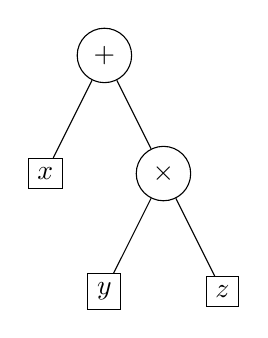
\begin{tikzpicture}
\node [circle,draw] {$+$}
  child {node [draw] {$x$}}
  child {
    node [circle,draw] (M) {$\times$}
    child {node [draw]{$y$}}
    child {node [draw]{$z$}}
  };
\end{tikzpicture}
\qquad\qquad
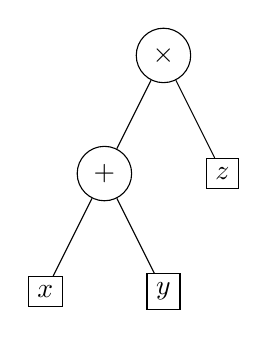
\begin{tikzpicture}
\node [circle,draw] {$\times$}
  child {
    node [circle,draw] (M) {$+$}
    child {node [draw]{$x$}}
    child {node [draw]{$y$}}
  }
  child {node [draw] {$z$}}
;
\end{tikzpicture}
\end{center}

Le regole di interpretazione della precedenza sono convenzionali
e possono esserci situazioni in cui non c'è una completa concordanza su come
una formula vada interpretata.
Quando le formule vengono rappresentate graficamente, inoltre,
anche la presentazione tipografica concorre nell'interpretazione
dell'ordine delle operazioni.
L'uso di spaziature, dimensioni e stili diversi oltre alla
posizione spaziale bidimensionale (linee di frazione, incolonnamenti)
intendono facilitare
l'interpretazione corretta dell'albero di valutazione riducendo
la necessità di utilizzare le parentesi.
\begin{comment}
Esempi di formule di dubbia interpretazione in
cui l'uso delle parentesi sarebbe invece auspicabile:
\[
  x/2\,y,\qquad
  \sin x \cdot 2, \qquad
  {e^x}^2, \qquad
  \frac{\displaystyle\frac{x}{y}}{z}.
\]
\end{comment}

\section{Calcolo dei predicati, quantificatori}

Possiamo pensare ai \myemph{predicati} come a proposizioni in cui
compaiono delle variabili.
Se una proposizione ha un valore di verità ben definito, il predicato
ha invece un valore di verità che dipende dal valore assegnato alle sue
variabili. Le variabili da cui dipende un predicato vengono chiamate
\myemph{variabili libere}. Le variabili libere possono venire \emph{chiuse}
(rese \emph{mute}) mediante operatori che agiscono
(estraendo un dato di sintesi) al variare della variabile su tutti i
suoi possibili valori.
Per quanto riguarda il calcolo proposizionale la chiusura delle variabili
di un predicato può essere fatta tramite i \myemph{quantificatori}
\emph{universale} $\forall$ (leggi: ``per ogni'') ed
\emph{esistenziale} $\exists$ (leggi: ``esiste'').
Ad esempio il predicato
$n>5 \Rightarrow n>m$ ha due variabili libere: $n$ ed $m$.
Possiamo chiudere la variabile $n$ con il quantificatore universale ottenendo:
\[
  \forall n \colon n>5 \Rightarrow n>m
\]
che è un predicato con una unica variabile libera $m$.
Il predicato può essere letto così: "per ogni $n$ se $n$ è maggiore di $5$ allora $n$ è anche maggiore di $m$."
Il valore di verità di questo
predicato dipende dal valore assegnato ad $m$.
Più precisamente il predicato è vero se $m\le 5$ ed è falso altrimenti.
La variabile $n$ è invece diventata muta, che significa che non ha più senso
assegnare dei valori alla variabile $n$ in quanto la verità di tale predicato non dipende più da $n$.

Per quanto riguarda l'intepretazione,
la proposizione ottenuta mediante un quantificatore universale
$\forall x\colon P(x)$ è vera se $P(x)$ è vera per ogni possibile valore
assegnato alla variabile $x$ ed è invece falsa se c'è anche un solo valore che
assegnato a $x$ rende falsa $P(x)$. Viceversa nella quantificazione
esistenziale $\exists x\colon P(x)$ si ottiene il vero nel caso ci sia almeno
un valore di $x$ che renda vera $P(x)$ e si ottiene il falso nel caso non ci sia
invece nessun valore di $x$ che renda vera $P(x)$.

Valgono in effetti le seguenti regole formali di scambio dei quantificatori con
la negazione logica:
\begin{align*}
  \neg \forall x \colon P(x) &\iff \exists x \colon \neg P(x)\\
  \neg \exists x \colon P(x) &\iff \forall x \colon \neg P(x).
\end{align*}
Osserviamo che queste relazioni corrispondono alle leggi di De Morgan per lo
scambio della negazione con gli operatori logici di congiunzione e disgiunzione.
Infatti l'operatore universale $\forall$ corrisponde ad una congiunzione logica
$\wedge$ su tutti i possibili valori del predicato,
così come l'operatore esistenziale
$\exists$ corrisponde ad una disgiunzione logica $\vee$.
Dal punto di vista mnemonico osserviamo che i simboli $\forall$ e $\exists$
si ottengono ruotando di 180 gradi le iniziali delle parole
\emph{All} ed \emph{Exists}.

Una variante dell'operatore esistenziale è l'operatore di unicità:
la proposizione $\exists! x\colon P(x)$ significa che esiste un \emph{unico} valore di $x$
che rende vero il predicato $P(x)$. Formalmente:
\[
  \exists!x\colon P(x) \iff \exists x\colon P(x)
  \wedge \neg \exists y\colon (y \neq x) \wedge P(y).
\]
Osserviamo che la precedente definizione utilizza il simbolo $\neq$ che è la
negazione dell'operatore di uguaglianza $=$ che verrà introdotto nella sezione
seguente.

\section{Teoria degli insiemi}

Fin'ora abbiamo presentato le regole logiche per la manipolazione dei valori di
verità dei predicati. Non abbiamo però ancora costruito nessun predicato né
tantomeno abbiamo introdotto gli oggetti che i predicati dovrebbero descrivere.

La teoria degli insiemi serve ad introdurre un \emph{universo} all'interno del
quale potremo identificare degli oggetti che possano rappresentare gli enti
matematici: numeri, funzioni, relazioni, insiemi.
Vedremo però che tutti questi enti matematici potranno essere ricondotti al
concetto di insieme: sarà dunque questo il concetto fondamentale che vogliamo
descrivere.

Intuitivamente gli \myemph{insiemi} sono collezioni di elementi.
Per costruire un sistema formale che descriva gli insiemi sarà sufficiente
introdurre l'unico predicato che mette in relazione un elemento con l'insieme
che lo contiene:
\[
  x \in A
\]
(leggi: ``$x$ è un elemento di $A$``).
Indicheremo con $\not \in$ la negazione
di questa relazione.
Dovremo indicare quali sono le regole formali che ci permetteranno di manipolare
questo tipo di formule.
Sarà utile poter costruire insiemi di insiemi, quindi in realtà nel predicato precedente
$x$ potrebbe a sua volta essere un insieme. Dunque, per semplicità, supporremo
che tutti gli oggetti siano insiemi.

A partire dalla relazione di \myemph{appartenenza} $\in$ potremo definire le altre
relazioni tra insiemi:
\begin{align*}
  A \subset B &\iff \forall x\colon (x \in A \Rightarrow x \in B)\\
  A \supset B &\iff \forall x\colon (x \in A \Leftarrow x \in B)\\
  A = B & \iff A\subset B \,\wedge\, B\subset A.
\end{align*}

Il simbolo $\subset$ rappresenta l'\myemph{inclusione} tra insiemi.
Osserviamo che in altri testi potrà essere invece utilizzato il simbolo $\subseteq$
per rappresentare la stessa relazione
rendendo esplicito il fatto che non si esclude che i due insiemi siano
uguali (inclusione larga).

La terza delle regole precedenti si chiama \emph{assioma di estensionalità}
e definisce il fondamentale concetto di \myemph{uguaglianza}.
Il nostro sistema formale sarà dotato di opportune regole di inferenza che
garantiscano che se due oggetti sono uguali
potranno essere liberamente sostituiti uno con l'altro in qualunque
altra formula. Questo garantisce la proprietà transitiva dell'uguaglianza.
Si definirà la \myemph{disuguaglianza} $\not =$ come negazione dell'uguaglianza.

Vogliamo anche introdurre le usuali operazioni di \myemph{intersezione} $A\cap B$,
\myemph{unione}  $A\cup B$ e \myemph{differenza} $A \setminus B$
che possono essere codificate dai seguenti assiomi:
\begin{align*}
  x \in A \cap B &\iff (x \in A \wedge x \in B)\\
  x \in A \cup B &\iff (x \in A \vee x \in B)\\
  x \in A \setminus B &\iff x \in A \wedge x \not \in B.
\end{align*}

Più in generale possiamo richiedere di poter fare l'unione o l'intersezione
di una famiglia $\F$ non vuota di insiemi (una \emph{famiglia} di insiemi non è altro che un insieme di insiemi):
\begin{align*}
  x \in \bigcap \F &\iff \forall A \in \F\colon x \in A \\
  x \in \bigcup \F &\iff \exists A \in \F\colon x \in A.
\end{align*}
Spesso si usano le seguenti notazioni più espressive:
\[
 \bigcap \F = \bigcap_{A \in \F} A,\qquad
 \bigcup \F = \bigcup_{A \in \F} A.
\]


Per avere un primo oggetto su cui agire definiamo l'\myemph{insieme vuoto},
denotato
dal simbolo $\emptyset$, mediante il seguente assioma
\[
\neg \exists x \colon x \in \emptyset.
\]
Osserviamo che le operazioni definite in precedenza, se applicate all'insieme vuoto,
non ci permettono di ottenere nuovi insiemi.
Per avere insiemi con un solo elemento introduciamo l'insieme \myemph{singoletto}
$\{ y \}$ cioè un insieme contenente un unico oggetto $y$:
\[
  x \in \{ y \} \iff x = y.
\]
A questo punto utilizzando l'unione possiamo già ottenere,
per elencazione,
insiemi con un numero
arbitrario (ma finito) di elementi, ad esempio:
\[
  \{a, b, c\} = \{ a \} \cup \{ b\} \cup \{c\}.
\]

Con le operazioni che abbiamo introdotto è già possibile descrivere infiniti insiemi
tra loro diversi. Ad esempio questi sono quattro insiemi diversi:
\[
 \emptyset,\quad
 \{ \emptyset \},\quad
 \{\{\emptyset\}, \emptyset\},\quad
 \{\{\emptyset\}, \{\{\emptyset\}\}\}
\]
mentre ognuno dei seguenti coincide con uno (quale?) dei precedenti:
\[
 \{\emptyset, \emptyset\},\quad
 \{\{\emptyset, \{\emptyset\}\}, \{\{\emptyset\}, \emptyset\}\}.
\]

Possiamo anche definire un insieme mediante una qualunque
proprietà che caratterizzi
i suoi elementi. Se $A$ è un insieme e $P(x)$ un predicato, allora
possiamo definire un insieme $B = \{x\in A\colon P(x)\}$ in modo
che si abbia
(\myemph{assioma di specificazione}):
\[
  b \in \{x\in A \colon P(x)\} \iff (b \in A) \wedge P(b).
\]
Osserviamo che viene richiesto a priori un insieme ambiente $A$ sul quale
viene ristretta la caratterizzazione. Questo significa che questo assioma non
può generare insiemi più grandi di quelli già esistenti.
Questo vincolo si è reso necessario per ovviare al paradosso di Russell.

\begin{paradox}[Russel]
Si consideri l'insieme
\[
  R = \{ x\colon x \not\in x\}.
\]
Allora $R\in R \iff R\not \in R$. Assurdo.
\end{paradox}

Il paradosso di Russel può essere espresso anche nel linguaggio naturale.
Una delle sue accezioni più note si chiama \emph{Paradosso del barbiere}
e si enuncia come segue. Il \emph{barbiere} è quella persona che fa la barba
alle persone che non se la fanno da se. Il barbiere si fa la barba da se?

Con la nostra impostazione l'insieme $R$ di Russel non può essere definito.
Se però fissiamo un insieme \emph{ambiente} $U$, possiamo definire il seguente:
\[
  R = \{ x \in U \colon x \not \in x\}.
\]
In tal caso abbiamo che $R\in R$ se e solo se $R\in U \wedge R\not \in R$.
In particolare se fosse $R\in R$ avremmo un assurdo. Ma non è invece
assurdo che $R\not \in R$, infatti in tal caso potrà essere (anzi, dovrà essere)
$R\not \in U$.
Non abbiamo ottenuto un paradosso, ma abbiamo scoperto che dato
un qualunque insieme $U$ esiste un insieme $R$ che non sta in $U$.
Questo significa che non esiste l'insieme \myemph{universo}, cioè un insieme che
contiene tutti gli insiemi. Osserviamo che l'insieme universo sarebbe il complementare
dell'insieme vuoto, e questo è il motivo per cui non è possibile definire
il complementare di un insieme ma ci si limita a definire la differenza tra insiemi.

La relazione $x\in x$ potrebbe di per se sembrare contraddittoria.
Come è possibile che un insieme contenga se stesso come elemento?
Se ad esempio avessimo $x=\{ x\}$ si avrebbe $x=\{\{x\}\} = \{\{\{ x\}\}\} \dots$
e così via in una discesa infinita che non avrebbe mai termine.
La possibilità che esistano insiemi di questo tipo è piuttosto fastidiosa ed è per questo
che si pone l'assioma di \emph{fondazione} (o di \emph{regolarità}) che afferma
in particolare che non esistono insiemi $x$ tali che $x\in x$.
Più in generale l'assioma di fondazione evita che sia possibile
costruire una catena discendente infinita di insiemi che siano
elemento uno dell'altro:
\[
  \dots \in x_n \in \dots \in x_2 \in x_1.
\]
Osserviamo però che anche assumendo che $x\not\in x$ sia sempre vera,
il paradosso di Russel rimane valido, in tal caso infatti
$R=\{x\colon x\not \in x\}$ dovrebbe contenere
tutti gli insiemi e quindi dovrebbe essere $R\in R$... che abbiamo escluso.

Un altro modo per dimostrare che è sempre possibile costruire un
insieme \emph{più grande} di un insieme dato si ottiene dall'insieme potenza
(che vediamo subito) tramite il teorema di Cantor (che vedremo più avanti).

L'assioma dell'insieme potenza, serve
a garantire l'esistenza del\-l'\myemph{insieme delle parti}.
Se $X$ è un qualunque insieme si può considerare $\P(X)$ come l'insieme dei
sottoinsiemi di $X$:
\[
 A \in \P(X) \iff A \subset X.
\]
L'insieme $\P(X)$ si chiama anche \emph{insieme potenza} e viene a volte indicato con $2^X$
in quanto se $X$ ha $n$ elementi allora $\P(X)$ ha $2^n$ elementi.
Ad esempio se $X=\{a, b, c\}$ ha tre elementi, l'insieme delle parti
ha otto elementi:
\[
 \P(X) = \{ \{\}, \{a\}, \{b\}, \{c\}, \{a,b\},
   \{a,c\}, \{b,c\}, \{a,b,c\}\}.
\]
Inteso che $\{\}=\emptyset$ osserviamo che l'insieme vuoto è sottoinsieme di
qualunque altro insieme (verificarlo tramite la definizione),
dunque appartiene sempre all'insieme delle parti.
L'insieme delle parti risulta fondamentale per poter esprimere
la \emph{logica del secondo ordine} ovvero la possibilità di poter
formulare predicati sui sottoinsiemi di un insieme invece che solamente
sui suoi elementi.

\section{Relazioni e funzioni}

Definiamo la \myemph{coppia ordinata} $(a,b)$ come un oggetto (un insieme,
visto che abbiamo deciso che tutti gli oggetti matematici sono insiemi) con
la seguente proprietà:
\begin{equation}\label{def:pair}
  (a,b) = (c,d) \iff a=c\, \wedge \,b=d.
\end{equation}
In particolare $(a,b) \neq (b,a)$ se $a\neq b$ cioè l'ordine dei due elementi
è importante.
Formalmente si potrebbe definire $(a,b)=\{\{a\}, \{a,b\}\}$,
si provi per esercizio a dimostrare che con questa definizione vale la
proprietà~\eqref{def:pair}.
Se $A$ e $B$ sono insiemi dati, l'insieme di tutte le coppie di elementi
presi il primo da $A$ e il secondo da $B$ si indica con $A \times B$ e si chiama
\myemph{prodotto cartesiano}:
\[
x \in A \times B \iff \exists a \in A, \exists b \in B\colon x = (a,b).
\]
Se $A$ ha $n$ elementi e $B$ ha $m$ elementi, il prodotto $A\times B$ ha $n\cdot m$
elementi. Ad esempio se $A=\{a,b,c\}$ ha tre elementi e $B=\{a,b\}$ ha due elementi,
il prodotto ha sei elementi:
\[
  A \times B = \{(a,a), (a,b), (b,a), (b,b), (c,a), (c,b)\}.
\]

Una \myemph{relazione} $R$ tra gli elementi di un insieme $A$
e gli elementi di un insieme $B$
non è altro che un sottoinsieme del prodotto cartesiano: $R\subset A \times B$.
Scriveremo $x R y$ quando $(x,y) \in R$.
Ad esempio su un insieme di numeri potremmo considerare come $R$ la relazione d'ordine
$\le$ per cui scriveremo $x \le y$ quando $(x,y)\in R$.
Le relazioni da un insieme in sé stesso possono eventualmente avere particolari caratteristiche
come essere: \emph{transitive} ($xRy \wedge yR z \implies x R z$),
\emph{simmetriche} ($xRy \implies yRx$),
\emph{riflessive} ($xRx$).
Come esercizio si provi a pensare alla relazione tra persone $xAy$
definita dalla frase "$x$ ama $y$".
Si consideri il significato delle proprietà transitiva, simmetrica
e riflessiva di tale relazione.

Possiamo pensare ad una coppia $(a,b)$ come ad una freccia che
parte da $a$ e arriva in $b$: $a \mapsto b$.
Potremmo scrivere più espressivamente $(a,b)\in R$ come
$a \stackrel{R}\mapsto b$.
In questo modo una relazione su $A\times B$
risulta essere un insieme di frecce che partono da elementi di $A$
ed arrivano su elementi di $B$. La rappresentazione che si ottiene prende
anche il nome di \emph{grafo orientato}.
Si provi ad interpretare \emph{graficamente} le proprietà
transitiva, simmetrica e riflessiva di un grafo.

Ogni relazione può essere \emph{invertita}\marginpar{relazione inversa}
semplicemente scambiando il ruolo
dei due insiemi $A$ e $B$. Se $R$ è una relazione e vale $x R y$
per la relazione inversa $R'$ si avrà
$y R' x$.
Pensando ad una relazione $R$ come un insieme di frecce
$x\stackrel R \mapsto y$,
la relazione inversa $R'$ risulta essere lo stesso insieme di frecce ma
con la direzione opposta $y\stackrel{R'} \mapsto x$.

Le relazioni che più ci interesseranno in questo corso sono le \myemph{funzioni}.
Le funzioni sono le relazioni \emph{univoche} cioè quelle relazioni $f$ in
$A\times B$ che
mandando (nel senso delle frecce) ogni elemento $a\in A$ in uno
ed un solo elemento
$b\in B$:
\[
\forall a\in A\colon \exists ! b\in B\colon a\stackrel{f}\mapsto b.
\]
Tale unico elemento $b\in B$ associato all'elemento $a\in A$ viene chiamato
\emph{immagine} di $a$ tramite $f$ e viene indicato con $b=f(a)$.
Una funzione definita da $A$ in $B$ si indica con $f\colon A \to B$. L'insieme
$A$ viene chiamato \myemph{dominio} e l'insieme $B$ \myemph{codominio}.

Le funzioni vengono spesso utilizzate per rappresentare delle trasformazioni.
Possiamo pensare ad una funzione come ad una scatola nera (un macinino)
a cui possiamo dare in pasto elementi dell'insieme $A$ (\emph{input})
e otteniamo come risposta elementi dell'insieme $B$ (\emph{output}).

Se l'output (codominio) di una funzione $f$
coincide con l'input (dominio) di una funzione $g$,
cioè se $f\colon A \to B$ e $g\colon B \to C$
possiamo comporre\marginpar{funzione composta}
le due funzioni per ottenere una funzione
$g\circ f \colon A \to C$:
\[
(g\circ f)(x) = g(f(x))\qquad
x \stackrel f \mapsto f(x) \stackrel g \mapsto g(f(x)).
\]

Vedremo come la composizione ci permette di costruire innumerevoli funzioni
componendo tra loro poche funzioni elementari, così come si può costruire un edificio
utilizzando semplici mattoni.
Ovviamente sarà importante conoscere a fondo
tutte le caratteristiche dei mattoni (proprietà delle funzioni elementari)
e sarà pure importante capire come tali proprietà si combinano quando mettiamo
insieme i diversi blocchi.

Uno dei problemi più importanti a
cui si può probabilmente ricondurre qualunque problema
matematico è quello dell'invertibilità di una funzione: data $f\colon A\to B$
trovare una funzione $g\colon B\to A$ tale che
se $x\stackrel f \mapsto y$ allora
$y \stackrel g\mapsto x$. Se ad esempio io so qual è la traiettoria di
un proiettile in funzione dell'angolo di tiro, mi chiedo quale angolo devo
scegliere per centrare un determinato bersaglio.
Oppure (altro esempio) data la funzione $f(x) = x^2$ (definita su un qualche insieme
numerico) dire se è possibile trovare $x$ tale che $f(x) = 2$
(definizione della radice quadrata).
Oppure ancora: se $x A y$ è la relazione ``$x$ ama $y$''
e se io sono $y$ sarei interessato a trovare gli $x$ tali che $x A y$.

Per poter invertire una funzione $f\colon A \to B$ abbiamo la necessità di verificare due
differenti proprietà: che per ogni $b\in B$ esista un elemento $a\in A$ tale che $f(a)=b$
(surgettività)
e che tale elemento $a$ sia unico (iniettività).
Più precisamente diremo che $f\colon A\to B$ è \myemph{surgettiva} se
\[
  \forall b\in B\colon \exists a \in A \colon f(a) = b
\]
ed è \myemph{iniettiva} se
\[
 \forall a\in A, \forall a'\in A\colon (f(a) = f(a') \implies a=a').
\]
Se una funzione $f\colon A \to B$ è iniettiva e surgettiva allora
si dice che $f$ è \myemph{bigettiva} o \myemph{invertibile}.
La funzione $g\colon B \to A$ che ad ogni
$b\in B$ associa l'unico $a\in A$ tale che $f(a)=b$ si chiama
\emph{funzione inversa} di $f$.
Tale funzione $g$ si indica anche con il simbolo $f^{-1}$ ed ha le proprietà
\[
  \forall x \in A\colon g(f(x)) = x, \qquad
  \forall y\in B\colon f(g(y)).
\]
La funzione inversa di $f$ è quindi anch'essa invertibile e l'inversa dell'inversa
è $f$ stessa: $(f^{-1})^{-1} = g^{-1} = f$.

Se $f\colon X\to Y$ è una funzione e se $A\subset X$ si definisce
l'insieme $f(A)$, chiamato \myemph{immagine} di $A$ tramite $f$ come:
\[
  f(A) = \{f(x)\colon x \in A\}
\]
se invece $B\subset Y$ si definisce l'insieme $f^{-1}(B)$, chiamato
\myemph{controimmagine} di $B$ tramite $f$ come:
\[
  f(B) = \{x\in A \colon f(x) \in B\}.
\]
Notiamo innanzitutto che la prima definizione non rientra esattamente
nell'assioma di specificazione ma è un modo più immediato per intendere
la seguente definizione che è invece perfettamente valida:
\[
  f(A) = \{y\in B \colon \exists x\in A \colon f(x) = y\}.
\]
Notiamo inoltre che questa definizione rappresenta un \emph{abuso di notazione}.
Infatti avevamo già dato una definizione per il simbolo $f(x)$.
Questa notazione va quindi utilizzata solo se il contesto rende chiaro il fatto
che $A$ va inteso come un sottoinsieme del dominio di $f$ e non come un elemento
di tale dominio.

Se $A=X$ è l'intero dominio della funzione
l'insieme $f(X)$ si chiama \emph{immagine di $f$}.
Possiamo allora osservare che una funzione $f\colon X \to Y$ risulta essere
surgettiva se e solo se $f(X) = Y$.
Se prendiamo un qualunque $y\in Y$ possiamo considerare l'insieme $f^{-1}(\{y\})$
che è sempre definito, anche se $f$ non fosse invertibile. Se tale insieme ha sempre
almeno un elemento significa che la funzione è surgettiva. Se tale insieme ha
sempre non più di un elemento significa che la funzione è iniettiva.
Se tale insieme ha sempre esattamente un elemento allora la funzione è invertibile
e si ha $f^{-1}(\{y\}) = \{f^{-1}(y)\}$.

Questo abuso di notazione
(inserire un insieme dove dovrebbe starci un singolo elemento)
potrà essere utilizzato anche con gli operatori infissi.
Una operazione, rappresentata ad esempio dal simbolo $+$, può essere pensata
come ad una funzione che agisce su una coppia di valori: $+\colon X\times Y \to Z$.
La notazione $x+y$ serve quindi ad abbreviare la notazione $+(x,y)$.
Anche in questo caso potrà capitare che al posto di $x$ o di $y$ o di entrambi,
si inserisca un insieme di valori:
\begin{align*}
   A + y &= \{x+y\colon x \in A\}, \\
   x + B &= \{x+y\colon y \in B\}, \\
   A + B &= \{x+y\colon x\in A, y \in B\}.
\end{align*}
In tutti questi casi il risultato è un insieme di valori, invece che un singolo
valore.

In maniera simile, questo abuso viene attuato anche con le relazioni.
Se ad esempio abbiamo
una relazione $x\le y$, e $A, B$ sono insiemi, si potrà intendere
che valgano le seguenti notazioni:
\begin{align*}
  x \le B &\iff (\forall y\in B\colon x\le y), \\
  A \le y &\iff (\forall x\in A\colon x \le y), \\
  A \le B &\iff (\forall x\in A, \forall y\in B\colon x\le y).
\end{align*}

\section{numeri naturali}

Abbiamo in precedenza affermato che tutti gli oggetti matematici di cui abbiamo
bisogno potranno essere rappresentati tramite gli insiemi.
Abbiamo visto, ad esempio, come le relazioni e le funzioni possono essere definite
utilizzando gli insiemi. Allo stesso modo possiamo procedere per definire i numeri
naturali: anch'essi saranno particolari insiemi.

Ci possono essere diversi modi per scegliere gli insiemi che definiscono i numeri
naturali, ma la definizione normalmente utilizzata è la seguente.
Si definisce il numero $0$ tramite l'insieme vuoto $\emptyset$ e si definisce
il successivo di $n$ come l'insieme $n^+ = n \cup \{ n \}$. Si avrà quindi
\begin{align*}
  0 &= \emptyset = \{\}, \\
  1 &= \emptyset^+ = 0 \cup \{0\} = \emptyset \cup \{0\} = \{0\}, \\
  2 &= \emptyset^{++} = 1 \cup \{1\} = \{0, 1\}, \\
  3 &= \emptyset^{+++} = 2 \cup \{2\} = \{0, 1, 2\},\\
  \vdots \\
  n &= \emptyset^{+\dots +} = \{ 0, 1, \dots, n-1\}, \\
  \vdots
\end{align*}
In particolare l'insieme che rappresenta il numero $n$ è un insieme di $n$
elementi (che sono i numeri più piccoli di $n$).

Osserviamo però che se è vero che riusciamo a definire i singoli numeri naturali,
nessuno degli assiomi che fin'ora abbiamo introdotto ci permette di definire
l'insieme di tutti questi numeri naturali.
In effetti, a bene riflettere, un \emph{universo} di insiemi formato solamente
dagli insiemi finiti (concetto che ancora non abbiamo definito ma che usiamo ora
in maniera intuitiva) soddisferebbe tutti gli assiomi fin'ora introdotti e non
potrebbe contenere l'insieme dei numeri naturali, che intuitivamente deve essere
infinito.
Sarà quindi necessario introdurre un nuovo assioma per il quale
introduciamo una apposita definizione.
Diremo che un insieme $A$ è \emph{induttivo} se $\emptyset \in A$
e $\forall n\in A\colon n^+\in A$.

Assioma dell'infinito:
\marginpar{assioma dell'infinito}
esiste un insieme $\NN$ \marginpar{$\NN$}
induttivo
tale che\footnote{%
In realtà sarebbe sufficiente garantire per assioma che esista un qualunque insieme induttivo
senza ulteriori specificazioni. Infatti se esiste almeno un insieme induttivo
$X$ chiameremo $\mathbb N$
l'intersezione degli insiemi induttivi contenuti in $X$. Si potrebbe infatti
verificare che l'intersezione di insiemi induttivi è induttivo ed essendo
l'intersezione contenuta in ogni insieme induttivo non può contenere strettamente
altri sottoinsiemi induttivi.
}
se $A\subset \NN$ è anch'esso induttivo allora $A=\NN$.
Chiameremo l'insieme $\NN$
\myemph{insieme dei numeri naturali}.

Essendo $\NN$ un insieme induttivo esso contiene tutti i numeri naturali come
li abbiamo definiti nel paragrafo precedente.
Inoltre $\NN$ è il più piccolo insieme induttivo
(non ci sono insiemi induttivi strettamente contenuti in $\NN$) e questo
serve a garantire che $\NN$ non contenga altri elementi al di fuori dei numeri
naturali.

Su $\NN$ possiamo definire la funzione $\sigma \colon \NN \to \NN$
tale che $\sigma(n) = n^+$. Formalmente si definisce $\sigma$ come relazione:
\[
  \sigma = \{(n,m) \in \NN \times \NN\colon m = n^+\}
\]
e si verifica facilmente che tale relazione è, effettivamente, una funzione.
Si può allora verificare che $\NN$ soddisfa le seguenti proprietà:
\begin{theorem}[assiomi di Peano]
Esistono $0\in \NN$
e $\sigma\colon \NN \to \NN$ tali che:
\begin{enumerate}
\item $\sigma$ è iniettiva;
\item non esiste $n\in \NN$ tale che $\sigma(n)=0$;
\item per ogni $A\subset \NN$ se
\begin{enumerate}
   \item $0\in A$;
   \item $n\in A \implies \sigma(n) \in A$;
\end{enumerate}
allora $A= \NN$.
\end{enumerate}
\end{theorem}

La proprietà induttiva dei numeri naturali permette di definire le funzioni su
$\NN$ utilizzando le \emph{definizioni per induzione}, come nel seguente.
\begin{theorem}\label{th:def_induction}[definizione per induzione]
Sia $X$ un insieme, $\alpha \in X$ e $g\colon \NN\times X \to X$.
Allora esiste un unica funzione $f\colon \NN \to X$ tale che
\[
\begin{cases}
  f(0) = \alpha,\\
  \forall n\in \NN\colon f(\sigma(n)) = g(n, f(n)).
\end{cases}
\]
\end{theorem}

Intuitivamente dopo aver definito $f(0) = \alpha$ si potrà definire
$f(1) = g(0, \alpha)$, $f(2) = g(1, f(1))$, $f(3) = g(2, f(2))$ etc.
Per la proprietà induttiva dei numeri naturali la funzione $f$ risulterà
definita univocamente su tutti i numeri naturali.

Con questo tipo di definizioni è possibile definire per induzione
l'operazione $+$ (addizione)
facendo in modo che valga la seguente proprietà:
\[
\begin{cases}
  n + 0 = n\\
  n + \sigma(m) = \sigma(n+m)
\end{cases}
\]
(in particolare si ottiene $\sigma(n)=n+1$)
e sarà possibile definire la moltiplicazione $\cdot$ in modo che
valga
\[
\begin{cases}
  n\cdot 0 = 0 \\
  n \cdot \sigma(m) = n\cdot m + n.
\end{cases}
\]
Si potrà poi verificare (cosa elementare ma non semplice)
che le operazioni così definite soddisfano le ben
note proprietà:
\begin{enumerate}
\item $n+0=n$, $n\cdot 1 = n$ (esistenza degli elementi neutri);
\item $n+m = m+n$, $n\cdot m = m\cdot n$ (proprietà commutativa);
\item $n\cdot (a+b) = n\cdot a + n\cdot b$ (proprietà associativa).
\end{enumerate}

Diremo che un numero $n\in \NN$ è divisibile per $m\in \NN$ se esiste $k\in \NN$
tale che $n = k \cdot m$. In tal caso scriveremo $k = n/m$.

Si potrà anche definire una relazione d'ordine $\le$ tramite la condizione
\[
  n \le m \iff \exists k \in \NN \colon m = n+k.
\]
La relazione $\ge$ si definisce come la relazione inversa di $\le$.
La relazione $<$ si
definisce richiedendo che sia $x\le y \land x\neq y$ e la relazione $>$
è definita come l'inversa di $<$.
Osserviamo che per come abbiamo costruito i numeri naturali (ci potrebbero essere
altre costruzioni che portano agli assiomi di Peano) si ha $n\le m \iff n \subset m$
e $n < m \iff n\in m$.

Come esempio di applicazione della definizione per induzione definiamo
il \emph{fattoriale} $n! = 1 \cdot 2 \dots n$ (il prodotto dei numeri naturali
da $1$ a $n$).
Per definire tale funzione
$\NN \to \NN$ in maniera rigorosa osserviamo che il prodotto dei numeri da $1$
a $n+1$ può essere definito come il prodotto dei numeri da $1$ a $n$ moltiplicato
per $n+1$. Imponendo poi che\footnote{%
E' chiaro che deve essere $1!=1$ e di conseguenza se vale $(n+1)! = (n+1)\cdot n!$
dovrà essere $0!=1$.
D'altra parte è naturale che il prodotto di un insieme vuoto di numeri sia
l'elemento neutro del prodotto, così come la somma di zero numeri è l'elemento
neutro della somma.
}
$0!=1$, si ottiene una caratterizzazione univoca:
\[
 \begin{cases}
  0! = 1 \\
  (n+1)! = (n+1) \cdot n!
 \end{cases}
\]
Si tratta di applicare il Teorema~\ref{th:def_induction}
con $X=\NN$, $\alpha = 1$, $g(n, x) = (n+1)\cdot x$ per garantire che esiste
una unica funzione $\NN\to\NN$, $n\mapsto n!$, che soddisfa queste proprietà.

In maniera simile si potrà definire per ogni $n,m \in \NN$ l'elevamento a potenza $n^m$
in modo che valga\footnote{%
Si noti che stiamo definendo $0^0=1$.
Alcuni testi lasciano indefinita questa operazione ma in realtà la formula
è giustificata dal fatto che $0^0$ è un prodotto di $0$ fattori e quindi,
come $0!$, deve valere $1$.
Questo viene confermato dal fatto che $n^m$ è il numero di funzioni da un
insieme con $m$ elementi in un insieme con $n$ elementi e
su un dominio vuoto è definita una unica funzione (la funzione vuota), anche
se il codominio è vuoto.
}
\[
\begin{cases}
  n^0 = 1\\
  n^{m+1} = n\cdot n^m.
\end{cases}
\]

La proprietà induttiva dei numeri naturali è equivalente al seguente.
\begin{theorem}[principio di induzione]
Sia $P(n)$ un predicato sui numeri naturali $n\in \NN$.
Se valgono le seguenti condizioni
\begin{enumerate}
\item $P(0)$ è vera
\item $P(n) \implies P(n+1)$
\end{enumerate}
allora $P(n)$ è vera per ogni $n\in \NN$.
\end{theorem}
%
\begin{proof}
Si consideri l'insieme $A=\{n\in \NN\colon \text{$P(n)$ è vera}\}$ e si
applichi il terzo assioma di Peano per verificare che $A=\NN$.
\end{proof}


\begin{exercise}
La somma $S(n) = 1 + 2 + \dots +n$
dei naturali da $1$ fino a $n$ può essere definita come quella unica funzione
che soddisfa le proprietà
\[
\begin{cases}
  S(0) = 0 \\
  S(n+1) = S(n) + (n+1).
\end{cases}
\]
Dimostrare che $S(n) = n \cdot (n+1) / 2$.
\end{exercise}

\begin{exercise}
Dimostrare che per la somma
$Q(n) = 1^2 + 2^2 + \dots + n^2$
(somma dei quadrati dei naturali da $1$ a $n$)
vale la formula
$Q(n) = n \cdot (n+1)\cdot (2n + 1) / 6$.
\end{exercise}

Potrà risultare utile utilizzare le seguenti varianti del principio di
induzione
\begin{theorem}[principio di induzione (variante)]
Sia $P(n)$ un predicato definito sui numeri naturali $n$
non inferiori a $n_0\in \NN$.
Se
\begin{enumerate}
\item $P(n_0)$ è vero
\item $P(n) \implies P(n+1)$ per ogni $n\ge n_0$
\end{enumerate}
allora $P(n)$ è vero per ogni $n\ge n_0$.
\end{theorem}

\begin{theorem}[principio di induzione forte]
Sia $P(n)$ un predicato definito sui numeri naturali $n\in \NN$.
Se
\begin{enumerate}
\item $P(0)$ è vero
\item $(\forall k\le n\colon P(k))\implies P(n+1)$
\end{enumerate}
Allora $P(n)$ è vero per ogni $n\in \NN$.
\end{theorem}

\begin{theorem}[buon ordinamento di $\NN$]
Se $A$ è un sottoinsieme non vuoto di $\NN$ allora esiste $a \in A$
tale che per ogni $x\in A$ si ha $a\le x$ (ovvero $a$ è minimo di $A$).
\end{theorem}
%
\begin{proof}
Supponiamo per assurdo che $A$ non abbia minimo e consideriamo l'insieme
$B=\{b\in \NN\colon b \le A\}$.
Chiaramente $0\in B$ in quanto $0\le \NN$. Se poi sapessimo che $n\in B$
allora $n\le A$. Non può essere $n\in A$ altrimenti $n$ sarebbe il minimo di $A$. Dunque $n < A$ e quindi $n+1 \le A$. Abbiamo quindi mostrato che se $n\in B$ anche $n+1\in B$. Per il principio di induzione deduciamo che $B=\NN$ e quindi $A$ sarebbe vuoto, cosa che abbiamo escluso per ipotesi.
\end{proof}



\section{cardinalità}

La teoria degli insiemi è nata con l'intento di formalizzare l'utilizzo degli
insiemi con infiniti elementi. Infatti finché gli insiemi hanno un numero finito
di elementi non ci sono dubbi sulle loro proprietà. L'utilizzo di insiemi con
infiniti elementi, invece, ci pone di fronte a questioni che possono sembrare
paradossali.

Per confrontare gli insiemi finiti è sufficiente contare il numero degli elementi.
Diremo che un insieme è \emph{più grande} se ha un numero di elementi maggiore.
Ma se gli insiemi sono infiniti, non siamo in grado di effettuare un conteggio
degli elementi. Possiamo però osservare che non è necessario contare il numero
di elementi per poter dire che due insiemi hanno la stessa numerosità.
Ad esempio in un parcheggio pieno posso dire che il numero di automobili
è uguale al numero di posti, senza dover contare né l'uno né l'altro ma semplicemente
osservando che c'è una corrispondenza biunivoca tra i posti e le auto. Faremo
lo stesso per confrontare insiemi infiniti.

Diciamo che due insiemi $A$ e $B$ sono equipotenti e scriveremo $\#A = \#B$
se esiste una funzione bigettiva $f\colon A \to B$.
Il simbolo $\#A$ si chiama \myemph{cardinalità} di $A$ e quindi due insiemi
sono equipotenti se hanno la stessa cardinalità.
In tal caso la funzione
$f$ è invertibile e l'inversa è anch'essa bigettiva,
quindi se $\#A = \#B$ risulta anche $\#B = \#A$.
Tramite la composizione è inoltre facile verificare che se $\#A = \#B$ e $\#B = \#C$
allora $\#A = \#C$.
Nel caso degli insiemi finiti vedremo che la cardinalità coincide con il
numero di elementi dell'insieme, ma ci potranno essere anche cardinalità
\emph{infinite}.

La relazione di equipotenza definisce il concetto di cardinalità, specificando
quali sono gli insiemi che hanno la stessa cardinalità. Possiamo anche mettere
un ordinamento tra gli insiemi, specificando che un insieme $A$ ha cardinalità
minore o uguale a quella di $B$, $\#A\le \#B$, se esiste una funzione
iniettiva $f\colon A \to B$. Scriveremo $\#A < \#B$ per indicare che
$\#A \le \#B$ ma non $\#A = \#B$ (dunque esistono funzioni iniettive da $A$ in $B$
ma nessuna di queste risulta essere surgettiva).

Non è difficile verificare che se esiste una funzione iniettiva $f\colon A\to B$
allora esiste anche una funzione surgettiva $g\colon B\to A$
(basta osservare che una funzione iniettiva $f$ è invertibile sulla propria
immagine $f\colon A \to f(A)$ e la funzione inversa può essere estesa a
tutto $B$ in maniera arbitraria).

Sugli insiemi finiti, di nuovo, questo concetto
si traduce con la corrispondente
disuguaglianza tra il numero degli elementi dei due insiemi.
Sugli insiemi infiniti, invece, abbiamo un concetto nuovo e i seguenti teoremi
non sono scontati.

\begin{theorem}[Cantor-Bernstein]
Se $\#A \le \#B$ e $\#B \le \#A$ allora $\#A = \#B$.
\end{theorem}
%
\begin{figure}
  \centering
  \input{CantorBernstein.tikz}
  \caption{
  Nella dimostrazione del teorema di Cantor-Bernstein
  $A$ è rappresentato da un quadrato e $B$ da un cerchio contenuto
  in $A$. L'immagine di $A$ in $B$ è rappresentata da un quadrato contenuto
  in $B$ e così via. La parte ombreggiata è l'insieme $D$.
  }
  \label{fig:omotetia}
\end{figure}
%
\begin{proof}
Per prima cosa al posto dell'ipotesi $\# B \le \#A$ prendiamo
l'ipotesi apparentemente più forte $B\subset A$.
Vedremo alla fine che questa ipotesi non ci fa perdere di generalità.

Essendo per ipotesi $\#A \le \#B$ esiste $f\colon A \to B$ iniettiva.
Intuitivamente l'idea è quella di definire l'insieme
\[
 D = (A\setminus B)  \cup f(A\setminus B) \cup f^2(A\setminus B) \cup \dots
\]
e di definire la biezione $\phi \colon A \to B$ mandando ogni "buccia"
$f^n(A\setminus B)$ in $f^{n+1}(A\setminus B)$ e lasciando fisso
il resto di $B$.

Per farlo in maniera rigorosa
consideriamo allora la famiglia di insiemi $\F = \{X \subset A \colon X \supset A \setminus B, f(X) \subset X\}$ e definiamo $D = \bigcap \F$.
Osserviamo che $A \in \F$ quindi $\F\neq \emptyset$.

E' facile verificare che $f(D) \subset D$ infatti dato $x\in D$ per ogni $X\in \F$ deve essere $x\in X$ ma allora $f(x) \in X$ (per come è definito $\F$), dunque $f(x) \in D$. In modo analogo si dimostra che $D\supset A\setminus B$ e dunque concludiamo che $D\in \F$.

Verifichiamo ora che $f(D)=D\cap B$. Da un lato se $x\in D$ allora
$f(x) \in f(D)\subset D$ e $f(x)\subset f(A)\subset B$ da cui $f(x) \in D\cap B$.
Dall'altro lato se $y\in D \cap B$ e non fosse $y \in f(D)$
allora potremmo considerare l'insieme $X=D\setminus\{y\}$
e osservare che $X\in \F$.
Infatti in primo luogo $X \supset A \setminus B$ in quanto $D$ ha questa proprietà e $y \in B$.
Inoltre dato qualunque $x \in X$ visto che $X\subset D$ allora
$f(x) \in f(D)$ e, per ipotesi,
$y\not \in f(D)$ dunque $f(x)\neq y$ da cui $f(x) \in X$.
Dunque $X\in \F$ ma allora dovrebbe essere $D\subset X$ mentre
per costruzione abbiamo $y\in D$ ma non in $X$.

% Avendo visto che $f(D)=D\cap B$ possiamo facilmente
% osservare che $f(A\setminus D) \subset A \setminus D$.
% Infatti $f(A\setminus D)\subset f(A)=B$ e quindi
% $f(A\setminus D)\cap D \subset D \cap B = f(D)$
% ma essendo $f$ iniettiva si deve avere
% $f(A\setminus D) \cap f(D)=\emptyset$.

Possiamo allora definire $\phi \colon A \to B$
\[
\phi(x) =
\begin{cases}
   f(x) & \text{se $x\in D$}, \\
   x & \text{altrimenti.}
\end{cases}
\]
Chiaramente $\phi$ è iniettiva in quanto $f$ è iniettiva e manda $D$ in $D$
e l'identità è iniettiva e manda $A\setminus D$ in $A\setminus D$.

Per dimostrare che $\phi$ è suriettiva consideriamo qualunque $y \in B$.
Se $y\not \in D$ allora $\phi(y)=y$.
Se invece $y\in D$ essendo $y\in D\cap B = f(D)$ esisterà $x\in D$ tale
che $\phi(x) = f(x) = y$.

Abbiamo dimostrato il teorema nel caso $B\subset A$.
Nel caso generale sappiamo che esiste $f\colon A\to B$ iniettiva
ed esiste $g\colon B\to A$ iniettiva. Definiamo $\tilde B=g(B)$ e
definiamo $\tilde f\colon A\to \tilde B$ tramite $\tilde f(x) = g(f(x))$.
Chiaramente $\tilde B\subset A$ e $\tilde f$ è iniettiva.
Dunque ci siamo ricondotti alle ipotesi particolari e sappiamo che esiste
$\tilde \phi \colon A \to \tilde B$ biettiva. Ma allora possiamo definire
$\phi\colon A\to B$ come $\phi(x) = g^{-1}(\tilde \phi(x))$.
Essendo $\tilde \phi(A)=\tilde B$ ed essendo $g\colon B\to \tilde B$
invertibile, risulta che anche $\phi$ sia biettiva.
\end{proof}

% Il seguente teorema è vero se assumiamo l'assioma della scelta.
% \begin{theorem}
% Almeno una delle due relazioni è valida: $\#A \le \#B$ o $\#B \le \#A$.
% \end{theorem}

Il seguente teorema è rilevante in quanto ci dice che gli insiemi infiniti
non sono sempre tra loro equipotenti, ma ci sono infiniti più grandi e più piccoli.
Osserviamo inoltre che il paradosso di Russel
ricalca la dimostrazione di questo teorema.

\begin{theorem}[Cantor]
Per qualunque insieme $X$ si ha $\# X < \# \P(X)$.
\end{theorem}
%
\begin{proof}
Che sia $\#X\le \#\P(X)$ è facile, basta prendere la funzione
$f\colon X\to \P(X)$ definita da $f(x) = \{x\}$ e verificarne
l'iniettività.

Per mostrare che $\# X \neq \#P(X)$ consideriamo
$f\colon X \to \P(X)$ una qualunque funzione
e definiamo l'insieme
\[
   C = \{x \in X \colon x \not \in f(x) \}.
\]
Vogliamo ora mostrare che non esiste un $c\in X$ tale che $f(c) = C$.
Infatti se tale $c$ esistesse, si avrebbe che la proposizione
$c\in C$ risulterebbe equivalente a $c\not \in C$ il che è impossibile.
Dunque la funzione $f$ non può essere surgettiva e questo significa che
non è $\#X \le \#P(X)$.
\end{proof}

\begin{exercise}
Utilizzando il principio di induzione dimostrare che se $\# A = n$ allora:
\begin{enumerate}
    \item $\# \P(A) = 2^n$;
    \item $\# \{f\colon A \to A\colon \text{$f$ biettiva}\} = n!$
      (le funzioni biettive di un insieme in sé si chiamano anche
      \emph{permutazioni}).
\end{enumerate}
\end{exercise}


\section{insiemi finiti/infiniti}

Diremo che un insieme $A$ ha $n$ elementi e scriveremo $\# A = n$,
se $A$ può essere messo in corrispondenza
biunivoca con l'insieme $n= \{0, \dots, n-1\}$ cioè se $\# A = \# n$.
Gli insiemi che possono essere messi in corrispondenza biunivoca con
un numero naturale si diranno \myemph{insiemi finiti}.
Tutti gli altri insiemi si diranno \myemph{insiemi infiniti}.

Si potrebbe dimostrare che non esistono insiemi infiniti di cardinalità
inferiore a quella di $\NN$, dunque un insieme $A$ è finito se $\# A < \#\NN$
ed è infinito se $\# A \ge \# \NN$.

Valgono poi i seguenti
\begin{theorem}[caratterizzazione degli insiemi finiti]
Sia $A$ un insieme. Le seguenti condizioni sono equivalenti:
\begin{enumerate}
\item $A$ è finito;
\item ogni funzione iniettiva $f\colon A \to A$ è suriettiva;
\item ogni funzione suriettiva $f\colon A \to A$ è iniettiva;
\end{enumerate}
\end{theorem}

\begin{theorem}[caratterizzazione degli insiemi infiniti]
Sia $A$ un insieme. Le seguenti condizioni sono equivalenti:
\begin{enumerate}
\item $A$ è infinito;
\item esiste $f\colon A\to A$ iniettiva ma non suriettiva;
\item esiste $f\colon A\to A$ suriettiva ma non iniettiva.
\end{enumerate}
\end{theorem}

\section{il teorema di incompletezza di G\"odel}

Il teorema di incompletezza di G\"odel afferma che ogni
sistema formale sufficientemente potente (diciamo che sia in grado di
descrivere i numeri naturali come abbiamo fatto noi) è incompleto.
La dimostrazione di tale risultato rivoluzionario richiederebbe un intero
corso di logica, ma possiamo solo accennare al fatto che l'idea della
dimostrazione consiste nell'associare un numero naturale ad ogni formula
del sistema, tradurre tutte le regole di inferenza in operazioni aritmetiche
in modo tale da poter formalizzare le dimostrazioni all'interno del sistema
stesso. Dopodiché ``basterà'' trovare un numero $G$ tale per cui
l'enunciato corrispondente a $G$ significa:
"l'enunciato corrispondente al numero $G$ non può essere dimostrato",
ovvero: "\emph{questo} enunciato non può essere dimostrato".
E' chiara l'analogia con il paradosso di Epimenide: "questa frase è falsa".

Si osservi che l'enunciato $G$ di G\"odel non parla direttamente di verità,
che è un concetto esterno al sistema formale
(dipende dal modello che noi diamo al sistema).
Ma se vogliamo attaccare un valore di verità ad ogni enunciato dovremo decidere
se $G$ è vero o falso. Se è vero avremmo un sistema in cui un enunciato vero
non può essere dimostrato e quindi tale sistema sarebbe incompleto.
Se invece $G$ è falso avremmo un sistema in cui un enunciato falso può essere
dimostrato e quindi tale sistema sarebbe \myemph{incoerente} (ci sono degli assiomi
falsi oppure delle regole di inferenza che permettono di dedurre enunciati falsi
a partire da enunciati veri).

\section{i numeri interi}

Sui numeri naturali $\NN$ sono definite le operazioni di addizione e moltiplicazione.
Risulta utile estendere $\NN$ in modo che ogni numero abbia anche un opposto, cioè in modo che per ogni $n$ esista $m$ tale che $n+m=0$.

\section{Appendice: Asse del tempo}
Asse del tempo:
\begin{itemize}
\item[-700] Epimenide
\item[-571] Pitagora
\item[-490] Zenone
\item[-384] Aristotele
\item[-367] Euclide
\item[1170] Fibonacci
\item[1564] Galileo
\item[1596] Des Cartes
\item[1815] Boole
\item[1845] Cantor
\item[1848] Frege
\item[1858] Peano
\item[1862] Hilbert
\item[1872] Russel
\item[1906] Godel
\item[1912] Turing
\end{itemize}

\section{Contributi}

Hanno segnalato errori e correzioni:
niccolo-p,
Antoine Venturini.
\end{document}
